\section{Auswertung}
\label{sec:Auswertung}

\subsection{Mittelwert}

Der Mittelwert $\mu$ wird im Allgemeinen über folgende Formel berechnet:

\begin{equation}
    \mu = \frac{1}{N} \sum_{n=1}^{N} x_n
\end{equation}
\\
$x_n$ sind die aus den Messungen berechneten Werte und $N$ ist die Anzhal der Werte. Die Standardabweichung von $D$ 
wird dabei wie folgt berechnet:
\\
\begin{equation}
    \sigma = \sqrt{\frac{1}{N-1}\sum_{n=1}^{N} (x_n -\mu)^2}
\end{equation}
\\
Das Mitteln der Werte aus der Tabelle \ref{tab:Messdaten} ergibt damit die Federkonstante:
\\
$D$\,=\,\num{2,9614+-0,0785}

\subsection{Lineare Ausgleichsrechnung}


    \begin{gather}
        F= m \cdot x + b \\ 
        m= \frac{\overline{x\cdot F}-\overline{x}\cdot \overline{F}}{\overline{x^2}-\overline{x}^2} \\ 
        b= \frac{\overline{F}\cdot \overline{x^2}-\overline{x\cdot F}\cdot \overline{x}}{\overline{x^2}-\overline{x}^2} 
    \end{gather}


\begin{figure}
    \centering
    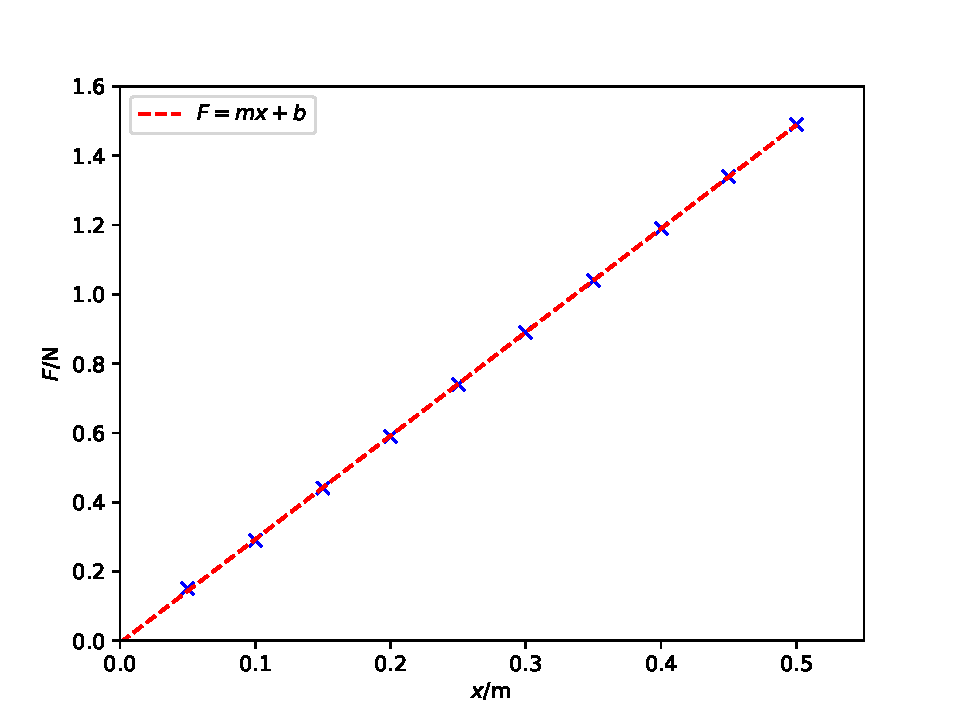
\includegraphics[width=\textwidth]{Python_dateien/Plot_Ausgleichsrechnung.pdf}
    \caption{Ausgleichsrechnung}
\end{figure}


